\documentclass{sig-alternate}
  \pdfpagewidth=8.5truein
  \pdfpageheight=11truein



%\usepackage{balance}
\usepackage[thmmarks]{ntheorem}

\usepackage{amsfonts}
\usepackage{amssymb,amsmath,latexsym}
\usepackage{enumerate}
\usepackage{listings}

\usepackage{multicol}
\usepackage{ifdraft}

\usepackage{graphicx,url}
\usepackage{graphics}
\usepackage{tikz}
\usetikzlibrary{shapes.geometric}
\usepackage{enumerate}
\usepackage{algorithm,algorithmic}

\usepackage{epstopdf}
\usepackage{array}
\usepackage{multirow}
\usepackage{rotating}
\usepackage{verbatim}

%%%%%%% OUR COMMANDS
\newcommand \com[1]{}


\newcounter{numberInTrivlist}

\newenvironment{numtrivlist}{\begin{list}{\rm \arabic{numberInTrivlist})} 
                                         {\usecounter{numberInTrivlist}
                                          \setlength{\leftmargin}{0pt}
                                          \setlength{\rightmargin}{0pt}
                                          \setlength{\itemindent}{12pt}
                                          \setlength{\listparindent}{0pt}}}
                            {\end{list}}


\def\P{\hbox{${\cal P}$}}


\def\bigV{\hbox{${\cal S}$}}
\def\V{\hbox{${S}$}}
\def\v{\hbox{${s}$}}
\def\MCDws{\ifmmode \mathit{COR\_D}\else \textit{COR\_D}\fi}

\def\bigA{\hbox{${\cal A}$}}
\def\Vabs{\hbox{${A}$}}

\def\bigO{\hbox{${\cal O}$}}

\def\useOpt{\hbox{${has\_opt}$}}
\def\G{\hbox{${\cal G}$}}


\def\B{\hfill{$\Box$}}
\def\A{\hbox{${\cal A}$}}
\def\K{\hbox{${\cal K}$}}
\def\T{\hbox{${\cal T}$}}
\def\O{\hbox{${\cal O}$}}
\def\F{\hbox{${\cal F}$}}
\def\D{\hbox{${\cal D}$}}
\newcommand{\bigP}{\mbox{I$\!$P}}



\theoremstyle{plain}
\theoremheaderfont{\normalfont\itshape}
\theorembodyfont{\normalfont}
\theoremseparator{.}
\theoremindent0cm
\theoremnumbering{arabic}
\theoremsymbol{\ensuremath{\Box}}
\newtheorem{definition}{Definition}[section]
\newtheorem{example}{Example}[section]
\newtheorem{lemma}{Lemma}[section]
\newtheorem{theorem}{Theorem}[section]
\newtheorem{coro}{Corollary}[section]


\renewcommand{\algorithmicrequire}{\textbf{Input:}}
\renewcommand{\algorithmicensure}{\textbf{Output:}}
\renewcommand{\algorithmicforall}{\textbf{for each}}
\newcommand{\ourremark}[3]{\noindent{{\footnotesize\sffamily\textcolor{#2}{#3\textsuperscript{#1}}}}}
\newcommand{\ja}[1]{\ourremark{\tiny JA}{red}{#1}}
\newcommand{\mhf}[1]{\ourremark{\tiny MHF}{blue}{#1}}

\newcommand{\ie}{\ifmmode \mathit{i.e.}\else \textit{i.e.}\fi}
\newcommand{\wrt}{\ifmmode \mathit{w.r.t.}\else \textit{w.r.t.}\fi}
\newcommand{\eg}{\ifmmode \mathit{e.g.}\else \textit{e.g.}\fi}
\newcommand{\lcp}{\ifmmode \mathit{isInst\_lcp}\else \textit{isInst\_lcp}\fi}
%\usepackage{authblk}



\begin{document}
%
% --- Author Metadata here ---
\conferenceinfo{SAC'13}{March 18-22, 2013, Coimbra, Portugal.}
\CopyrightYear{2013} % Allows default copyright year (2002) to be over-ridden - IF NEED BE.
\crdata{978-1-4503-1656-9/13/03}  % Allows default copyright data (X-XXXXX-XX-X/XX/XX) to be over-ridden.
% --- End of Author Metadata ---

\title{Sampling Negative Examples for Predicting Prokaryotic Promoters}
\subtitle{[Extended Abstract]}

\numberofauthors{1}

\author{
\alignauthor 
%Eduardo G. Gusm\~{a}o\\
%     \affaddr{{Center of Informatics, Federal University of Pernambuco}}\\
%       \affaddr{{Recife, Brazil}}\\
%% 2nd. author
%\and
%\alignauthor Marcilio C. P. de Souto\\
%       \affaddr{{Department, University}}\\
%       \affaddr{{Province, Country}}\\
%       \email{{mcps@cin.ufpe.br}}
}

\maketitle
\begin{abstract} 
Supervised learning methods have been successfully used to build classifiers for the identification of promoter regions. The classifier is often built from a dataset that has examples of promoter (positive) and non-promoter  (negative)  regions.  Thus, a careful selection of the data  used for constructing and testing a promoter finding algorithm is a very important issue.  In this context, whereas experimentally known promoter regions can safely be assumed to be positive training instances,   since  definite knowledge whether a given region is not a promoter  is not generally available,  negative instances are not straightforward to be obtained. To make the problem more complex, for the case of promoter, there is not  a univocal definition of what a negative instance is. As a consequence, depending on which definition of non-promoter region one assumed to  build  the data, such a choice  could affect  significantly the performance of the classifier and/or yield a biased estimate of the performance. We present an empirical study of the effect of this kind of problem for promoter prediction in {\it E. coli}. As far as we are concerned, up to now, there is no such a  kind of study for the context of prokaryotic promoter prediction.
%\keywords{sampling, prokaryotic promoter prediction, supervised learning}
\end{abstract}


\section{Introduction}
\label{sec:intro}

Identification of promoters is very important since they play a central role in transcription~\cite{maston2006}. Furthermore, as the complexity of organisms increase, the number of events that composes their regulatory network and the DNA regions reserved to perform control of gene expression rise significantly. This  makes wet-lab low-throughput methods not sufficient to perform annotation of DNA control elements efficiently in a genome-wide manner. Consequently, many computational approaches have been suggested to overcome the low-throughput issue, each of which has their strengths and weaknesses.

Promoter prediction in prokaryotes is often modeled as a binary classification task, in which the method has to learn to discriminate between promoter (positive) and non-promoter  (negative)  regions. These samples are frequently  nucleotide sequences (primary sequence) or features extracted from them. In early studies, Norton~\cite{norton1994} made interesting observations about the methodological issues concerning sequence extraction from consensus genomes. He also developed a probabilistic method to predict promoters by evaluating uncertainty in the training data. Helmann~\cite{helmann1995} analyzed 236 {\it B. subtilis} promoters recognized by ${\sigma }^{{A}}$-RNA polymerase and evidenced interesting characteristics concerning conserved positions and dinucleotide frequency patterns. More recently, Dhar \cite{dhar2010} reviewed the use of features such as curvature, bendability and stability to try to build more accurate  classifiers. Wu et al~\cite{wu2011} improved the prediction accuracy with a method that considered the correlations between nucleotides at the construction of position weight matrices representing the promoters. In another interesting work, Avila e Silva~\cite{avila2011} made neural networks simulations based both on the primary sequences (nucleotide sequences)  and other  features expressing sequences in terms of their free energy.

Independently of the  type of attribute used to represent the instances in the dataset, primary sequence and/or its features, one methodological issue that researchers have to account for is the construction/choice of the negative instances.  Nowadays, there are many experimentally known promoter regions that can safely be assumed to be positive training instances. In contrast,  it is experimentally complex to prove that a sequence does not to contain a promoter. As a result, negative examples have been obtained in alternative ways, each one of them leading to different ``definitions" for what a negative example is. For instance,  the authors in~\cite{bland2010} simply take random fragments that are not included in the positive dataset. In another work, the authors  extract random sequences from coding and non-coding regions~\cite{gordon2003}.  There are also examples in which fragments from a related organism, such as phages, are taken as negatives instances~\cite{towell1993,monteiro2005}. 

Depending on which definition of non-promoter region one assumed to  build  the data, such a choice  could affect  significantly the performance of the classifier and/or yield a biased estimate of the performance. In this paper, as our main contribution, we present an empirical study of the effect of this kind of problem using  the promoter prediction in {\it E. coli} as  the case study. As far as  we are concerned, up to know, there is no such a kind of analysis for the context of prokaryotic promoter prediction.


\section{Related Works}
\label{sec:related}

The problem with negative sampling is common in many  areas of bioinformatics such as prediction of microRNA (miRNA) target mRNAs, regulatory networks, protein-protein interactions, non-coding RNA finding, among others \cite{bandyopadhyay2009,cerulo2010,park2011,wang2006}. For instance, in miRNA target studies most methods suffer from high rates of false positives or false negatives because systematic identification of mRNAs not proven to be target of miRNAs is still not addressed properly, compelling current machine learning methods to rely on artificially generated negative examples for training \cite{bandyopadhyay2009}. Regulatory networks modeling and protein-protein interactions share the problem that definite knowledge is typically not available that a given pair of genes, proteins or other products under study do not interact \cite{cerulo2010,park2011}.

There are also studies approaching how to deal with the problem. One of the strategies that has been showing to provide good results is the use of positive instances only with a robust statistical background \cite{cerulo2010,wang2006,yousef2008}. In \cite{wang2006}, for instance, the authors presented an algorithm, Positive Sample only Learning (PSoL), that combined with SVM created a powerful tool for finding non-coding RNA genes. Other interesting way to deal with the problem  is the establishment of benchmarks, standardizing the definitions of negative examples and providing high-quality datasets. In the context of protein-protein interactions, for example,  a repository (Negatome Database) was constructed containing proteins that have high probability not to interact~\cite{smialowski2010}. We believe that these standardizations are great contributions to bioinformatics areas where negative samples are hard to define or obtain.


\section{Materials and Methods}
\label{sec:methods}

We perform an empirical study of impact of the choice of negative examples in the performance of  classifiers built for the task of   promoter prediction, using a dataset of  {\it E. coli} as case study.  Such a problem is investigated from the perspective in which the primary sequences (sequences of nucleotides) are given directly as input to the learning algorithm, as well as in the context in which the input for the learning algorithms are features extracted from the sequences. More specifically, we use the variable-window Z-curve (vw Z-curve) feature extraction method presented in~\cite{song2011a}.

In terms of machine learning techniques, for both context, we apply  a rule based system (decision trees) and statistical learning systems such as naive bayes classifier and  support vector machines.  Additionally, for the scenario in which the attributes are the features extracted with  vw Z-curve  method, we apply the partial least squares algorithm as in the work in~\cite{song2011a}.  All the learning methods used in our study were obtained from the Matlab.

Next, we present the datasets that we use in the experiments. Then, we briefly introduce the variable-window Z-curve feature extraction method. Finally, we discuss the methodology used to evaluate the experiments.

\subsection{Datasets}

As previously mentioned, the main focus  of this study is the evaluation of the impact of specific biases associated with  the use of the different definitions  of negative samples when building a dataset. As general guideline to construct our data, we use the work in~\cite{gordon2003}. 

The 812 sequences representing the positive dataset, that is, the promoters, were obtained from RegulonDB~\cite{gama2008}. We use promoters from {\it E. coli} that contain motifs recognized by ${\sigma }^{{19}}$, ${\sigma }^{{24}}$, ${\sigma }^{{28}}$, ${\sigma }^{{32}}$, ${\sigma }^{{38}}$, ${\sigma }^{{54}}$ and ${\sigma }^{{70}}$. All sequences have 80bp length spanning [TSS-60,TSS+19]. Only experimentally verified promoters are used, that is,  promoters predicted by transcription initiation mapping or RNA polymerase footprinting, which, according to RegulonDB criteria, are the methods that provides strong evidence. Hereafter, we refer to this dataset as {\tt POS}.

With respect to the data representing the negative examples, as will be explained in the following, we define different sets taking as basis if the sequences come from coding regions, non-coding regions or from random segments of the genome.  For certain cases,  some sequences needed to be extracted from {\it E. coli } complete genome and coding regions. This was accomplished  using  the database at  NCBI ~\cite{ncbi2012} for {\it E. coli } K-12 MG1655. All the negative sequences, as in the case of the positive ones, consist of 80 nucleotides.\\

\noindent
{\bf Coding Negative Examples}. As pointed in~\cite{gordon2003}, 81\% of known {\it E. coli} K-12 TSS are located in the intergenic non-coding regions and 19\% in the coding regions. Based on this,  we decided to include the coding data present in~\cite{gordon2003,song2011a}. Basically, they picked at random   836 genomic sequences  from the start ORFs of      {\it E. coli}  known coding regions. We denote such dataset as {\tt COD1}. For reasons that we will discuss later,  we propose a second coding dataset ({\tt COD2}) consisting of 826 sequences randomly drawn from any part of the coding regions, not only from  the start of the ORFs as in~\cite{gordon2003,song2011a}. 

\noindent
{\bf Non-coding Negative Examples}. Like~\cite{gordon2003,song2011a}, we also decided to include in our analysis the non-coding examples from a random sample of non-coding convergent intergenic spacers~\cite{palleja2009}. This dataset, which will refer to as {\tt NCOD}, consists of 825 sequences. 

\noindent
{\bf Random Negative Examples}. Following the methodology in Bland et al \cite{bland2010}, we created these data  from sequences chosen at random. In order to do so,  we extracted  at random   825  fragments from the {\it E. coli}  genome, but with the constraint that these sequences cannot have any overlap with the sequences from the positive set ({\tt POS}).  Compared to the previous two cases case, as they are chosen at random, the sequences  could belong to coding or non-coding regions. Such  dataset will be denoted by {\tt RAND}.

\noindent
{\bf Miscellaneous Negative Examples}. The methodology used to generate each of  the previous negative datasets, with exception, to a certain degree,  of {\tt RAND}, will not include in the data sequences from different parts of the genome. For example, {\tt COD1} and {\tt COD2} will not present any fragment from  non-coding convergent intergenic spacers ({\tt NCOD}). However, from a practical point of view, when one scans a genome looking for promoters, the systems will have as input fragments from any part of the genome. Motivated by this,  we propose to create two additional negative datasets. The first dataset consists of a random sampling of 50\% of the sequences from {\tt COD1} and  50\% of the sequences from  {\tt NCOD}, which we  will be denote by  {\tt MIX1}. The second dataset, denoted by {\tt MIX2},  follow the same procedure, but using  {\tt COD2} and {\tt NCOD}. 

\noindent
{\bf Control Negative Examples}. To put the results into perspective, we created a ``synthetic" negative dataset. Such a dataset is composed of  812 sequences that were generated completely at random, that is, they were not picked from any part of a genome. We will denote this dataset as {\tt CTRL}.\\

The datasets previously defined can be seen as important representative of positive and negative examples used in the literature of prokaryotic promoter prediction analysis. A summary of all these datasets is presented in Table~\ref{table:data}. The first column represents the name of the dataset, the second column provides a short description, the third column denotes the number of sequences in the respective dataset, and the remaining columns represent the frequencies of the nucleotides in each dataset. 

\renewcommand{\multirowsetup}{\centering}
\begin{table*}

\caption{List of datasets \label{table:data}}
\begin{center}
    \renewcommand{\arraystretch}{1.2}
    \begin{tabular}{>{\centering\arraybackslash} m{1.0cm} 
                    >{\centering\arraybackslash} m{5.0cm} 
                    >{\centering\arraybackslash} m{1.5cm} 
                    >{\centering\arraybackslash} m{1.0cm}
                    >{\centering\arraybackslash} m{1.0cm}
                    >{\centering\arraybackslash} m{1.0cm}                    
                    >{\centering\arraybackslash} m{1.0cm}}
        \hline
            Dataset & Description & Nr. Seq. & A & C & G & T \\
        \hline
            {\tt POS}  & Known promoters & 812 & 29.04 & 20.48 & 20.00 & 30.48 \\
        \hline
           {\tt COD1} & Start of coding regions & 836 & 26.62 & 22.29 & 24.88 & 26.21 \\
        \hline
            {\tt COD2} & Random part of coding region & 836 & 24.19 & 24.58 & 27.21 & 24.02 \\
        \hline
           {\tt  NCOD} & Non coding region & 825 & 23.94 & 25.01 & 26.78 & 24.27 \\
        \hline
            {\tt RAND} & Random non-promoter region & 812 & 24.46 & 25.79 & 25.34 & 24.41 \\
        \hline
            {\tt MIX1} & 50\% COD1 + 50\% NCOD & 830 & 25.47 & 23.35 & 25.83 & 25.35 \\
        \hline
            {\tt MIX2} & 50\% COD2 + 50\% NCOD & 830 & 24.02 & 24.69 & 27.14 & 24.15 \\
        \hline
           {\tt CTRL} & Completely random sequences & 812 & 25.14 & 25.02 & 25.20 & 24.64 \\
        \hline
    \end{tabular}
\end{center}
\vspace{-1.0cm}
\end{table*}

 

\subsection{Variable-window Z-Curve Feature Extraction}

The variable-window Z-curve (vw Z-curve) feature extraction, developed by Song~\cite{song2011a}, consists of a variation of the regular Z-curve approach proposed by Zhang~\cite{zhang1997}. They can both be  used to extract numerical features from a nucleotide sequence. The main idea of the original Z-curve theory is that a 3D curve (or point) representation for a DNA sequence can be created in the sense that each can be uniquely reconstructed given the other. The original Z-curve is calculated from the frequencies of the four bases occurring in the sequence and consider three main components: distribution of purine/pyrimidine, distribution of amino/keto and distribution of strong/weak H-bonds. The regular Z-curve parameters are only derived from the frequencies of mononucleotides occurring in a DNA sequence. Song claims this is a limitation for the case of  promoter recognition and  modified this idea by introducing a variable-window that allows the point to be in a much higher dimension.  More formally, the vw Z-curve method  can be defined as follows~\cite{song2011a}.

Let $ S_{w}^{i} $ be a string constructed by picking $ w $ elements from the set $ \{A,C,G,T\} $ with order and repetition, where $ w $ is defined as the window length and $ i = 1, ..., w^{4} $. For example, when $ w = 2 $, $ S_{2}^{1} = AA $, $ S_{2}^{2} = AC $, ..., $ S_{2}^{16} = TT $. Let the frequency of the pattern $ S_{w}^{i}X $ be denoted by $ p\left(S_{w}^{i}X\right) $, where $ X \in \{A,C,G,T\} $. The following equation shows the uniform definition of the vw Z-curve variables.

\begin{equation}
    \begin{array}{lcl}
        x_{S_{w}^{i}} & = & [p\left(S_{w-1}^{i}A\right) + p\left(S_{w-1}^{i}G\right)] - \\
                      &   & [p\left(S_{w-1}^{i}C\right) + p\left(S_{w-1}^{i}T\right)] \\[0.3cm]
        y_{S_{w}^{i}} & = & [p\left(S_{w-1}^{i}A\right) + p\left(S_{w-1}^{i}C\right)] - \\
                      &   & [p\left(S_{w-1}^{i}G\right) + p\left(S_{w-1}^{i}T\right)] \\[0.3cm]
        z_{S_{w}^{i}} & = & [p\left(S_{w-1}^{i}A\right) + p\left(S_{w-1}^{i}T\right)] - \\
                      &   & [p\left(S_{w-1}^{i}C\right) + p\left(S_{w-1}^{i}G\right)] \\[0.3cm]
        \text{where}  & : & \quad w \in \mathbb{N} \quad \text{and} \quad i = 1, 2, ..., 4^{w-1} \\
    \end{array} 
    \label{eq:xdef}
\end{equation}

For example, given a certain sequence (independently of its length, 80 or 200 nucleotides), if we  generated its respective  vw Z-curve,  with $ w = 1, ..., 6 $, such a sequence will be represented by a real valued vector with 4095 attributes ---  each window $w$  generates $ 3*4^{w-1} $ features. 

\subsection{Evaluation}

In order to compare the accuracy of each dataset we will perform a 10-fold cross validation using four supervised learning techniques: Support Vector Machine (SVM), Naive Bayes classifier   (NB), Decision Trees (DT) and Partial Least Squares (PLS)~\cite{song2011a,mitchell1997}. In every fold, classifiers are generated by training the supervised learners with a combination of the positive dataset ({\tt POS}) with every other negative dataset.

We  investigate the performance of classifiers in two different scenarios. The first scenario regards the performance results  yielded by the usual 10-fold cross validation procedure. For example, given the dataset ({\tt POS} + {\tt COD1}), by applying 10-fold cross validation, we can build  10 SVMs. Then, the result will be the average of the performance of each one of these SVMs tested with its respective testing set drawn from ({\tt POS} + {\tt COD1}).

In the second scenario, for instance, we test classifiers generated with a given dataset with  different negative examples sets.   For example, given the dataset ({\tt POS} + {\tt COD1}), by applying 10-fold cross validation, we build  10 classifiers. Then, we can test the performance of these classifiers with, for instance, the dataset {\tt POS} + {\tt NCOD}. Obviously that, in terms of the  positive examples, the performance will be the same for both cases. However, in terms of negative examples, as the classifiers  were trained with {\tt COD1}, they could have more difficulty in correctly assigning examples coming from completely different dataset ({\tt NCOD}).

In summary, in terms of challenging the classifiers, the first scenario should  be ``easier"  than the second one, since the testing examples are taken from the same distribution used to create the classifiers. Hereafter, we refer to these two scenarios, respectively,  as {\bf Case study 1} and {\bf Case study 2}.

We used three metrics to evaluate the accuracy of the classifiers: correct rate (Cr), sensitivity (Sn), specificity (Sp). Table~\ref{table:acc}  presents these statistics, assuming TP, FP, TN and FN are, respectively, the number of true positives, false positives, true negatives and false negatives.  In order to evaluate whether the variation in accuracy between different methods were significant, we applied a paired t-test using  a confidence level of 95\%.

%\renewcommand{\multirowsetup}{\centering}
\begin{table}

\caption{Statistics used for accuracy assessment \label{table:acc}}
\begin{center}
    \renewcommand{\arraystretch}{1.2}
    \begin{tabular}{>{\centering\arraybackslash} m{3.0cm} 
                    >{\centering\arraybackslash} m{2.0cm} 
                    >{\centering\arraybackslash} m{2.0cm}}
        \hline
            Correct Rate & Sensitivity & Specificity \\
        \hline
            \multirow{2}{*}{$\dfrac {TP+TN}{TP+FP+TN+FN}$}       &
            \multirow{2}{*}{$\dfrac {TP}{TP+FN}$}                &
            \multirow{2}{*}{$\dfrac {TN}{TN+FP}$}                \\
            & & \\
        \hline
    \end{tabular}
\end{center}
\vspace{-1.0cm}
\end{table}


\section{Experiments and Results}
\label{sec:results}

In our experiments we use (1) the primary sequence datasets (categoric attributes) and (2)  datasets whose attributes  and characteristics were extracted by the vw Z-curve method (numeric attributes).  For the latter,  following the guidelines in~\cite{song2011a}, we  first generated their respective  vw Z-curve datasets,  with $ w = 1, ..., 6 $.  This yields 4095 feature for each sequence. We, then,  selected 300 features from the 4095 using the PLS-based feature selection described in~\cite{song2011a}. This number of selected features was chosen based on the accuracies reported by Song under different number of features for {\it E. coli } datasets. 


 In terms of machine learning techniques, for both context, we apply  Decision Trees (DTs),  Naive Bayes classifier (NB) and  Support Vector Machines (SVMs).  Also, for the scenario in which the attributes are the features extracted with  vw Z-curve  method, we apply the Partial Least Squares (PLS) algorithm as in the work in~\cite{song2011a}. In addition, a right-tailed paired t-test at the 5\% significance level is performed in order to access the statistical significance of the results obtained. All the learning methods used in our study were obtained from the Matlab. We use the default parameters for DTs, NB and PLS. For the case of SVMs, after performing some  pre-experiments, we chose to use the polynomial kernel with the exponent set to 3, the complexity factor (C) set to 0.5, and least square as optimization technique. \\

\noindent
{\bf Case study 1}: the performance assessment with the usual 10-fold cross validation procedure \\

Figure~\ref{fig:seq} illustrates the results for the  usual  10-fold cross validation procedures applied to  SVM. Such a figure presents results  only for primary sequence datasets (nucleotide sequences). At first glance, one can observe that  the SVM  performed better than the other classifiers. Except for {\tt COD1}, the specificity of the SVM  was usually lower than its sensitivity. Differently, for  NB and DT , the difference between  sensitivity and specificity was not large. 

Looking at Figure~\ref{fig:seq},  the most noticeable result is the large values for the statistics obtained by training and testing with {\tt COD1}. This can be explained by the fact that {\tt COD1}  was created by extracting  sequences from  the start of gene ORFs. That is, such a negative example  dataset is the only one that has a highly conserved motif (ATG).  We will present a more detailed discussion of this specific bias later in this section. 

\begin{figure*}

\vspace{0.0cm}
    \centering
    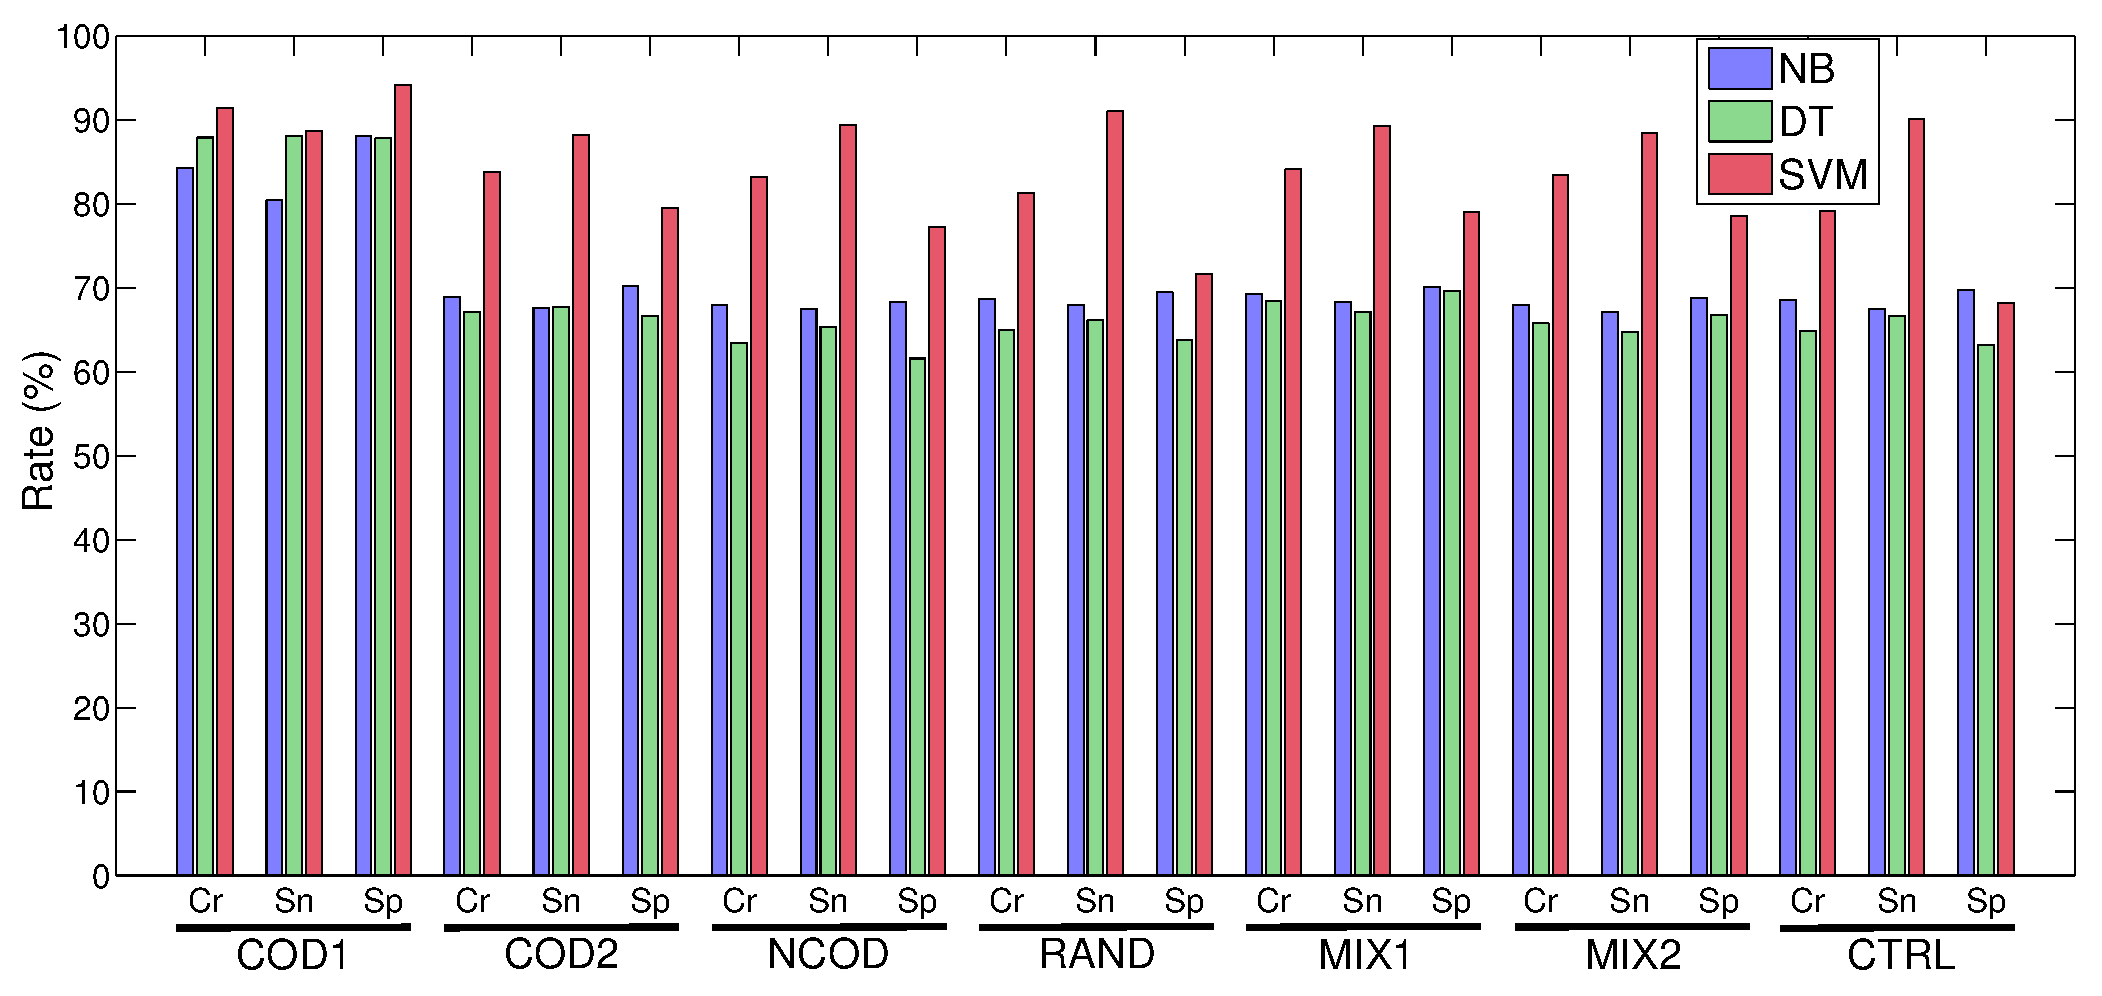
\includegraphics[width=1.0\textwidth]{Figs/Fig1.eps}
    \caption{Result of 10-fold cross validation for  SVM applied to the primary sequence datasets \label{fig:seq}}
   \vspace{0.0cm}
\end{figure*}

Now, we turn our analysis to the same data, but, instead of using directly the primary sequences, we  consider as attributes  the features extracted via the vw  Z-curve. The results are shown in Figure~\ref{fig:zcurve}.  NB, SVM and PLS performed similarly for all the datasets, with a slight advantage for SVM in most cases. On the other side, DT had much lower rates in comparison to the other methods. As DT is not very appropriate to deal with numeric attributes, this is an expected result. 

Comparing Figures~\ref{fig:seq} and~\ref{fig:zcurve}, one can observe slightly lower results for {\tt COD1}  (and {\tt MIX1}, which consists of 50\% of {\tt COD1}). However, no great variations can be observed. Methods based on the use of different  features(properties)  extracted from the primary sequence as attributes, instead of using directly the sequence,  have been gained popularity.  These results also suggests that, in addition to improving predication power by providing a wider range of information, this methodology does not suffer from biases originating from sequence alignment issues. \\

\begin{figure*}
\vspace{0.0cm}
    \centering
    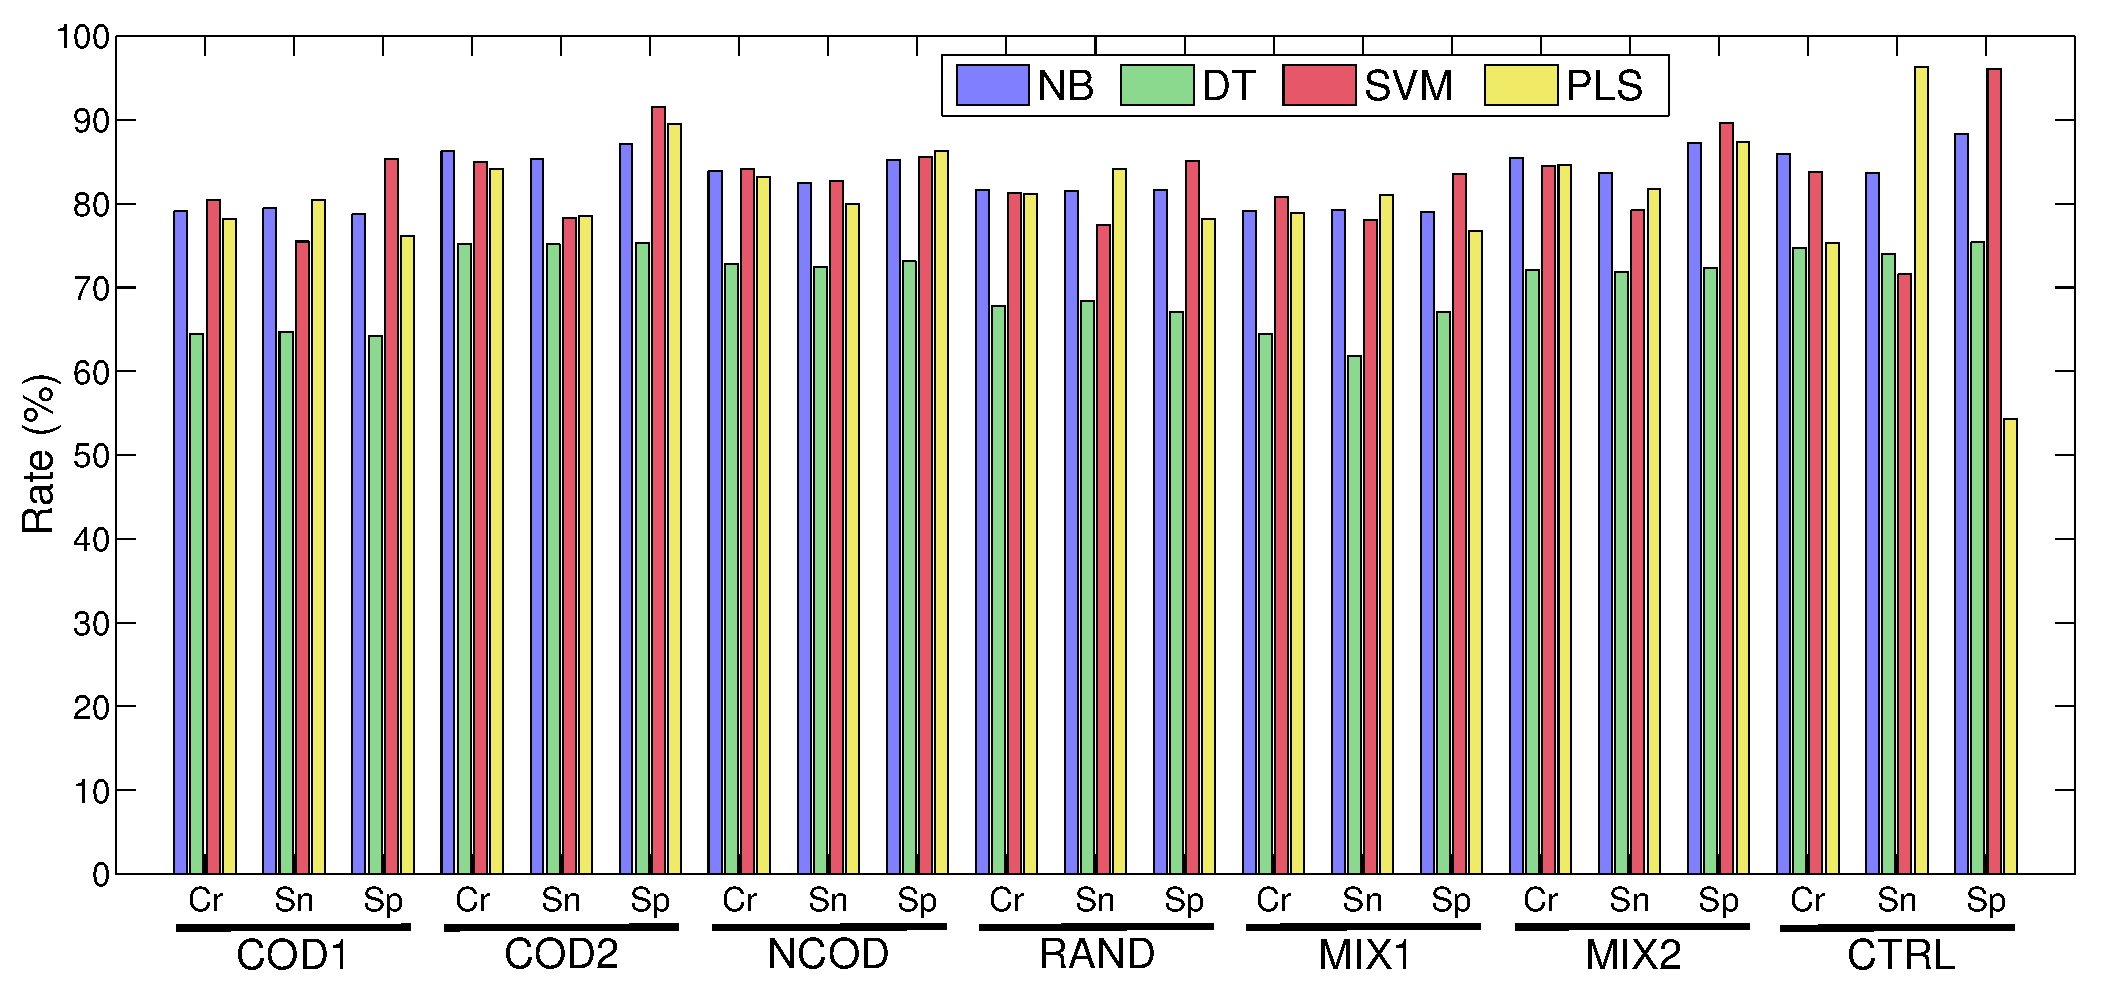
\includegraphics[width=1.0\textwidth]{Figs/Fig2.eps}
    \caption{Result of 10-fold cross validation for  SVM applied to vw Z-curve datasets using 10-fold cross validation  \label{fig:zcurve}}
   
\vspace{0.0cm}
\end{figure*}

\noindent
{\bf Case study 2}: the performance assessment with different negative datasets \\

Table~\ref{table:spe} provides specificity rates obtained by the application of SVM classifier to all combinations of training and testing sets. The upper part of the table regards the primary sequences datasets, whereas the lower part contains the results for vw Z-curve datasets. 

For primary sequence datasets, the bias generated by the presence of ATG motif in {\tt COD1} is now evident:  the specificity rates suffer a dramatic drop when {\tt COD1} is used as a training set and other datasets are used as testing set (first row of the upper part of the table). An interesting result is the fact that, for certain contexts, we can observe higher rates for testing with other dataset rather than the one used to build the classifier. For example, in the case of {\tt MIX2}, the classifiers presented better performance when tested either with {\tt COD2} and {\tt NCOD}. Since the application of novel methodologies will be done in a much noisier environment that the controlled 10-fold cross-validation, this could be seen as an evidence  that using multiple datasets is essential for any study.

In addition to the training bias, the use  of {\tt COD}1 also makes clear a testing bias that can be seen by verifying the low specificity rates when training with other datasets and testing with {\tt COD1} --- (first column of the upper part of the table). At this context, mixing datasets methodology has proven to minimize  this kind of bias, though  it is still noticeable its preference for its own instances when testing.

\begin{table*}
\caption{Specificity for training and testing with SVM classifier --- different  test sets \label{table:spe}}
\begin{center}
    \renewcommand{\arraystretch}{1.2}
    \begin{tabular}{|>{\centering\arraybackslash} m{0.5cm} 
                    |>{\centering\arraybackslash} m{0.5cm} 
                    |>{\centering\arraybackslash} m{1.2cm} 
                    |>{\centering\arraybackslash} m{1.2cm} 
                     >{\centering\arraybackslash} m{1.2cm} 
                     >{\centering\arraybackslash} m{1.2cm} 
                     >{\centering\arraybackslash} m{1.2cm} 
                     >{\centering\arraybackslash} m{1.2cm} 
                     >{\centering\arraybackslash} m{1.2cm} 
                     >{\centering\arraybackslash} m{1.2cm}|}
        \cline{4-10}
            \multicolumn{1}{c}{} & \multicolumn{1}{c}{} & \multicolumn{1}{c|}{} & \multicolumn{7}{c|}{\centering Testing } \\
        \cline{4-10}
            \multicolumn{1}{c}{} & \multicolumn{1}{c}{} & \multicolumn{1}{c|}{} & COD1 & COD2 & NCOD & RAND & MIX1 & MIX2 & CTRL \\
        \hline
            \multirow{14}{*}{\begin{sideways}Training\end{sideways}} & \multirow{7}{*}{\begin{sideways}Sequence\end{sideways}} & COD1 &
            94.14 & 39.43 & 38.30 & 35.83 & 68.80 & 41.93 & 31.26 \\
            &  & COD2 &
            52.79 & 79.55 & 78.08 & 75.11 & 64.07 & 87.39 & 69.93 \\
            &  & NCOD &
            50.36 & 77.98 & 77.21 & 72.87 & 73.33 & 87.87 & 68.81 \\
            &  & RAND &
            47.98 & 75.73 & 73.67 & 71.67 & 58.39 & 74.80 & 66.06 \\
            &  & MIX1 &
            95.25 & 67.61 & 82.39 & 63.88 & 79.04 & 75.76 & 58.40 \\
            &  & MIX2 &
            54.90 & 87.79 & 87.83 & 73.88 & 70.40 & 78.55 & 69.47 \\
            &  & CTRL &
            48.22 & 73.74 & 74.76 & 71.93 & 59.75 & 74.27 & 68.23 \\
        \cline{2-10}
            & \multirow{7}{*}{\begin{sideways}Z-curve\end{sideways}} & COD1 &
            85.29 & 91.91 & 84.88 & 82.14 & 91.84 & 88.29 & 72.98 \\
            &  & COD2 &
            71.44 & 91.51 & 85.16 & 80.11 & 77.84 & 92.66 & 62.13 \\
            &  & NCOD &
            61.69 & 84.84 & 85.58 & 80.50 & 79.72 & 92.08 & 56.43 \\
            &  & RAND &
            69.00 & 87.39 & 89.25 & 85.10 & 78.84 & 88.81 & 69.77 \\
            &  & MIX1 &
            87.33 & 91.06 & 93.60 & 84.96 & 83.49 & 91.96 & 68.15 \\
            &  & MIX2 &
            68.76 & 94.00 & 91.85 & 80.25 & 79.57 & 89.64 & 64.84 \\
            &  & CTRL &
            63.18 & 75.73 & 79.52 & 79.27 & 70.17 & 76.12 & 96.06 \\    
        \hline
    \end{tabular}
\end{center}
\vspace{-0.5cm}
\end{table*}

In contrast to what we have discussed previously for primary sequence datasets,   the results of the Z-curve datasets  did not present the training bias generated by the conserved ATG in {\tt COD1}. Indeed, the behavior observed was the opposite. When training with {\tt COD1}, the values  for testing with {\tt COD2}, {\tt MIX1} and {\tt MIX2}  were moderately larger. This unexpected fact led us to conduct a more careful  analysis of the structure of these datasets. 

In order to do so,  we calculated the centroid (average vector) for each dataset in Table~\ref{table:data}. Then, we computed the euclidean distance between the centroids of each dataset  --- inter-dataset distance.   Based on this, a probable explanation for the ``inverse" {\tt COD1}  bias for Z-curve datasets is that the distance between the centroids of {\tt POS} and {\tt COD2}  is greater than that of between {\tt POS} and {\tt  COD1} (respectively, 2.77 and 2.13), while the distance between {\tt COD1} and {\tt COD2 } is much lower (1.62).  From a geometrical point of view,  whatever the decision boundary between {\tt POS} and {\tt COD1} is, this same boundary would be able to correctly classify examples from {\tt COD2}, which are closer to the instance in {\tt COD1}, but more distant from the examples in {\tt POS}.  \\

\noindent
{\bf Discussion} \\

Having analyzed the results of our experiments, we point the fact that when applying any methodology in real biological datasets, the learners face data that do not behave so well as in wet-lab guided experimental pipeline. ``Real world" data consists of general and specific biases and noises that may differ depending on simple actions such as parameter setting. In addition, there are several  types of methodological details that, when incorrectly treated, often leads to biased results. For instance, the dataset {\tt COD1}, used in~\cite{gordon2003,song2011a}, contains a conserved motif that, in terms of methods that use primary sequence as input,  lead the classifiers generated to classify incorrectly  negative examples coming from different distributions. 

Moreover,  since the goal of any genome-wide prediction technique is to run a classifier  and retrieving the regions that are more likely to be enriched for what is expected it to be, using coding and non-coding negative samples in separate does not necessarily address the actual problem. In this context, although our analysis has shown no significant bias related to the {\tt RAND} dataset, the original definition made in~\cite{bland2010} excluded, from the negative dataset, regions within 50bp of the TSS. These regions are known to have lower SIDD profile levels, which is a characteristic of a promoter region. Thus,  in generating their negative examples in this way, they somehow prevent  getting into the dataset segments of genomes that could make the classification, in this context of SIDD profile features,  harder. In fact, as demonstrated by in our experiments,  when considered out of the SIDD profile context, picking sequences  at random from the genome could lead to a dataset that  provides a pessimistic view of the classifiers generated.

In summary, we suggest that in studies that the negative examples are hard to determine or supporting evidence is not present, the accuracy assessment should be done spanning the largest possible number of scenarios. This includes training and testing with different datasets corresponding to different interpretations of negative dataset, generating other datasets when feasible such as combinations of these datasets, assessing the accuracy through a wider range of statistics and exploring other methodological possibilities such as semi-supervised learning and positive only prediction, even when slight modifications to the original classifiers needed to be performed.


\section{Final Remarks}
\label{sec:final}

In this work, we discussed a number of different biases and misinterpretations that often occurs in bioinformatics studies concerning the use of supervised learners when negative instances are hard to obtain or define. To support our discussion we created two evaluation scenarios where a 10-fold cross-validation was applied to 14 different datasets, composed of sequences and features extracted from these sequences, using four machine learning methods. We showed specific and general biases that happened under these circumstances and suggested evaluation criteria to assess the real performance of novel algorithms over a wide range of bioinformatics fields.

This study can be further expanded to encompass other evaluation scenarios. For example, other features extracted from the sequences can be used such as SIDD profile~\cite{bland2010} or DNA stability based on free energy~\cite{avila2011}. Other possibility is the use of a wider number of classifiers, allowing for a detailed discussion on the specific bias of each learner. One can also compare other approaches, such as non-supervised, semi-supervised or positive sample only learning,  to the classical supervised methodology~\cite{cerulo2010,wang2006,yousef2008}.

\subsubsection*{Acknowledgments.} We would like to thank Ivan G. Costa and Tha\'{i}s G. do R\^{e}go for sharing some valuable information and for making helpful suggestions.

\vspace{0.5cm}
%%%%%%%%%%%%%%%%%%%%%%%%%%%%%%%%%%
\bibliographystyle{plain}
\bibliography{References}
%%%%%%%%%%%%%%%%%%%%%%%%%%%%%%%%%%
\end{document}